\section{Undetermined Coefficients [25\%]}
States $u_i$ are given at three nodes in a non-uniform, one-dimensional grid, as shown below.  Using the method of undetermined coefficients, derive the most accurate formula for $du/dx$ at node 2, and give the order of accuracy, with respect to $h$, of your formula.


\begin{figure}[h]
    \centering
    

\tikzset{every picture/.style={line width=0.75pt}} %set default line width to 0.75pt        

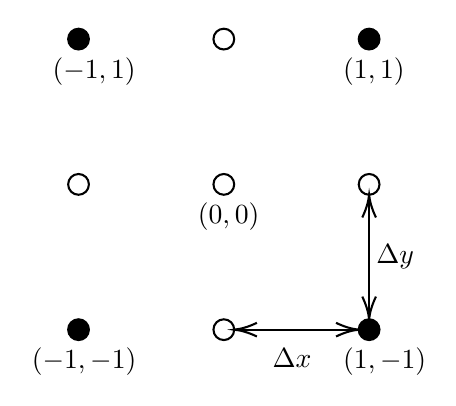
\begin{tikzpicture}[x=0.75pt,y=0.75pt,yscale=-1,xscale=1]
%uncomment if require: \path (0,300); %set diagram left start at 0, and has height of 300

%Shape: Circle [id:dp06682781228078438] 
\draw  [fill={rgb, 255:red, 0; green, 0; blue, 0 }  ,fill opacity=1 ] (240,65) .. controls (240,62.24) and (242.24,60) .. (245,60) .. controls (247.76,60) and (250,62.24) .. (250,65) .. controls (250,67.76) and (247.76,70) .. (245,70) .. controls (242.24,70) and (240,67.76) .. (240,65) -- cycle ;
%Shape: Circle [id:dp2823555602353238] 
\draw  [fill={rgb, 255:red, 0; green, 0; blue, 0 }  ,fill opacity=1 ] (380,65) .. controls (380,62.24) and (382.24,60) .. (385,60) .. controls (387.76,60) and (390,62.24) .. (390,65) .. controls (390,67.76) and (387.76,70) .. (385,70) .. controls (382.24,70) and (380,67.76) .. (380,65) -- cycle ;
%Shape: Circle [id:dp6222623809561607] 
\draw  [fill={rgb, 255:red, 0; green, 0; blue, 0 }  ,fill opacity=1 ] (380,205) .. controls (380,202.24) and (382.24,200) .. (385,200) .. controls (387.76,200) and (390,202.24) .. (390,205) .. controls (390,207.76) and (387.76,210) .. (385,210) .. controls (382.24,210) and (380,207.76) .. (380,205) -- cycle ;
%Shape: Circle [id:dp14694556239035372] 
\draw  [fill={rgb, 255:red, 0; green, 0; blue, 0 }  ,fill opacity=1 ] (240,205) .. controls (240,202.24) and (242.24,200) .. (245,200) .. controls (247.76,200) and (250,202.24) .. (250,205) .. controls (250,207.76) and (247.76,210) .. (245,210) .. controls (242.24,210) and (240,207.76) .. (240,205) -- cycle ;
%Shape: Circle [id:dp8106200964793124] 
\draw   (310,135) .. controls (310,132.24) and (312.24,130) .. (315,130) .. controls (317.76,130) and (320,132.24) .. (320,135) .. controls (320,137.76) and (317.76,140) .. (315,140) .. controls (312.24,140) and (310,137.76) .. (310,135) -- cycle ;
%Shape: Circle [id:dp06002439214257249] 
\draw   (380,135) .. controls (380,132.24) and (382.24,130) .. (385,130) .. controls (387.76,130) and (390,132.24) .. (390,135) .. controls (390,137.76) and (387.76,140) .. (385,140) .. controls (382.24,140) and (380,137.76) .. (380,135) -- cycle ;
%Shape: Circle [id:dp22749598300585605] 
\draw   (310,65) .. controls (310,62.24) and (312.24,60) .. (315,60) .. controls (317.76,60) and (320,62.24) .. (320,65) .. controls (320,67.76) and (317.76,70) .. (315,70) .. controls (312.24,70) and (310,67.76) .. (310,65) -- cycle ;
%Shape: Circle [id:dp8588323743643862] 
\draw   (240,135) .. controls (240,132.24) and (242.24,130) .. (245,130) .. controls (247.76,130) and (250,132.24) .. (250,135) .. controls (250,137.76) and (247.76,140) .. (245,140) .. controls (242.24,140) and (240,137.76) .. (240,135) -- cycle ;
%Shape: Circle [id:dp5234863402795684] 
\draw   (310,205) .. controls (310,202.24) and (312.24,200) .. (315,200) .. controls (317.76,200) and (320,202.24) .. (320,205) .. controls (320,207.76) and (317.76,210) .. (315,210) .. controls (312.24,210) and (310,207.76) .. (310,205) -- cycle ;
%Straight Lines [id:da3521724505838646] 
\draw    (322,205) -- (378,205) ;
\draw [shift={(380,205)}, rotate = 180] [color={rgb, 255:red, 0; green, 0; blue, 0 }  ][line width=0.75]    (10.93,-3.29) .. controls (6.95,-1.4) and (3.31,-0.3) .. (0,0) .. controls (3.31,0.3) and (6.95,1.4) .. (10.93,3.29)   ;
\draw [shift={(320,205)}, rotate = 0] [color={rgb, 255:red, 0; green, 0; blue, 0 }  ][line width=0.75]    (10.93,-3.29) .. controls (6.95,-1.4) and (3.31,-0.3) .. (0,0) .. controls (3.31,0.3) and (6.95,1.4) .. (10.93,3.29)   ;
%Straight Lines [id:da034995775783171146] 
\draw    (385,142) -- (385,198) ;
\draw [shift={(385,200)}, rotate = 270] [color={rgb, 255:red, 0; green, 0; blue, 0 }  ][line width=0.75]    (10.93,-3.29) .. controls (6.95,-1.4) and (3.31,-0.3) .. (0,0) .. controls (3.31,0.3) and (6.95,1.4) .. (10.93,3.29)   ;
\draw [shift={(385,140)}, rotate = 90] [color={rgb, 255:red, 0; green, 0; blue, 0 }  ][line width=0.75]    (10.93,-3.29) .. controls (6.95,-1.4) and (3.31,-0.3) .. (0,0) .. controls (3.31,0.3) and (6.95,1.4) .. (10.93,3.29)   ;

% Text Node
\draw (231,72.4) node [anchor=north west][inner sep=0.75pt]    {$( -1,1)$};
% Text Node
\draw (301,142.4) node [anchor=north west][inner sep=0.75pt]    {$( 0,0)$};
% Text Node
\draw (371,72.4) node [anchor=north west][inner sep=0.75pt]    {$( 1,1)$};
% Text Node
\draw (221,212.4) node [anchor=north west][inner sep=0.75pt]    {$( -1,-1)$};
% Text Node
\draw (371,212.4) node [anchor=north west][inner sep=0.75pt]    {$( 1,-1)$};
% Text Node
\draw (337,212.4) node [anchor=north west][inner sep=0.75pt]    {$\Delta x$};
% Text Node
\draw (387,162.4) node [anchor=north west][inner sep=0.75pt]    {$\Delta y$};


\end{tikzpicture}

    \caption{Undetermined coefficients non-uniform, one-dimensional grid.}
\end{figure}


\vspace{-0.5in}
\begin{align*}
    \shortintertext{First I will consider forward, backward, and central differences\newline \textbf{\underline{Forward Difference:}}}
    \sum_{i=2}^{3}\ a_i u_i & = a_2u_2 + a_3u_3\\
    u_3 & \approx u_2 + 2hu' + \frac{1}{2}(2h)^2u'' + \frac{1}{6}(2h)^3u'''\\
    \frac{du}{dx}|_{2} & = a_2u_2 + a_3 \left( u_2 + 2hu' + \frac{1}{2}(2h)^2u'' + \frac{1}{6}(2h)^3u'''\right)\\
    \shortintertext{This gives the following systems of equations,}
    a_2 + a_3 & = 0,\quad 2ha_3  = 1\ \text{Solving gives,}\ a_3 = \frac{1}{2h}, \quad a_2 = -\frac{1}{2h}\\
    \frac{du}{dx}|_{2} & \approx \frac{1}{2h}(u_3 - u_2)\\
    a_3 2h^2u'' & \rightarrow \frac{1}{2h}2h^2u'' \rightarrow hu'',\quad \mathcal{O}(h) \rightarrow \text{First-Order}\\
    \shortintertext{\textbf{\underline{Backward Difference:}}}
    \sum_{i=1}^{2}\ a_i u_i & = a_1u_1 + a_2u_2\\
    u_1 & \approx u_2 + (-h)u' + \frac{1}{2}(-h)^2u'' + \frac{1}{6}(-h)^3u'''\\
    \frac{du}{dx}|_{2} & = a_1(u_2 + (-h)u' + \frac{1}{2}(-h)^2u'' + \frac{1}{6}(-h)^3u''') + a_2u_2\\
    a_1 + a_2 & = 0, \quad -ha_1  = 1,\ \text{Solving gives,}\ a_1 = -\frac{1}{h}, \quad a_2 = \frac{1}{h}\\
    \frac{du}{dx}|_{2} & \approx \frac{1}{h}(u_2 - u_1)\\
    a_1\frac{h^2}{2}u'' & \rightarrow -\frac{1}{h}\frac{h^2}{2}u'' \rightarrow -\frac{h}{2}u'', \quad \mathcal{O}(h) \rightarrow \text{First-Order}
\end{align*}


\pagebreak
\pagestyle{fancy}
\restoregeometry


\vspace{-0.5in}
\begin{align*}
    \shortintertext{\textbf{\underline{Central Difference:}}}
    \sum_{i=1}^3 & = a_1 u_1 + a_2u_2 + a_3u_3\\
    \shortintertext{Using the expressions for $u_1$ and $u_3$ from forward and backward gives,}
    & a_1(u_2 - hu' + \frac{1}{2}h^2u'' - \frac{1}{6}h^3u''')+\ldots\\
    & a_2u_2+\ldots\\
    & a_3(u_2+2hu' + 2h^2u'' + \frac{4}{3}h^3u''')\\
    \shortintertext{This gives the following systems of equations,}
    & a_1 + a_2 + a_3 = 0\\
    & -ha_1 + 2ha_3 = 1\\
    & \frac{1}{2}h^2a_1 + 2h^2a_3 = 0\\
\end{align*}

\vspace{-0.75in}
\begin{align*}
    \shortintertext{Solving for $a_1,\ a_2,\ a_3$ gives,}
    a_1 = -\frac{2}{3h},\quad & a_2 = \frac{1}{2h}, \quad a_3 = \frac{1}{6h}
    \shortintertext{This gives that the approximation is,}
    \frac{du}{dx}|_2 & \approx \frac{1}{6h}\left(u_3 + 3u_2 - 4u_2\right)\\
    \shortintertext{Finding the order of accuracy can be done by,}
\end{align*}

\begin{gather*}
    \left(a_1 \frac{1}{2}h^2 + a_32h^2\right)u''\\
    \left(-\frac{2}{3h}\frac{1}{2}h^2 + \frac{1}{6h}2h^2\right)u''\\
    \left(-\frac{1}{3}h + \frac{1}{3}h\right)u'' = 0u''\\
    \shortintertext{Need to go higher,}
    \left(a_1\left(-\frac{1}{6}\right)h^3 + a_3\left(\frac{4}{3}\right)h^3\right)u'''\\
    \left(\frac{2}{3h}\frac{1}{6}h^3 + \frac{1}{6h}\frac{4}{3}h^3\right)\\
    \rightarrow \left(\frac{h^2}{9} + \frac{2}{9}h^2\right)u''' \rightarrow \frac{h^2}{2}u'''
\end{gather*}


\begin{fminipage}{0.8\linewidth}
    \textbf{Thus, a central order difference is more accurate $\bf \mathcal{O}(h^2)$, meaning that it is second-order accurate and is more accurate than forward or backward differences (with them being first-order). The expression for $\bf du/dx$ at node 2 is given below.}
\end{fminipage}

\begin{equation*}
    \boxed{\frac{du}{dx}|_2 \approx \frac{1}{6h}\left(u_3 + 3u_2 - 4u_2\right)}
\end{equation*}
